%!TEX root=../document.tex

\section{Ergebnisse}
Da der erste Versuch nicht funktionierte, wurde auf eine Realisierung in JavaEE gesetzt mit Unterstützung von \verb|Spring Boot|, \verb|Spring Security|, \verb|Spring Data JPA| und der Datenbank \verb|HSQL|. Es wurde mit folgendem Tutorial gearbeitet:

\href{https://hellokoding.com/registration-and-login-example-with-spring-security-spring-boot-spring-data-jpa-hsql-jsp/}{https://hellokoding.com/registration-and-login-example-with-spring-security-spring-boot-spring-data-jpa-hsql-jsp/}

Das Endergebnis ist ein RESTful Webservice bei welchem man sich einloggen und registrieren kann und mit einer Willkommensnachricht begrüßt wird. 

\subsection{Allgemein}
Zuerst mussten gewisse Themengebieten recherchiert werden. Vor allem das Themengebiet \verb|Hibernate| musste von Grund auf gelernt und verstanden werden. Folgend werden einige Themen erklärt beziehungsweise Begriffe definiert. 

\subsubsection{Hibernate}

src: \href{https://howtoprogramwithjava.com/hibernate-persistence-beginners/}{https://howtoprogramwithjava.com/hibernate-persistence-beginners/}


Hibernate ''steht'' zwischen objektorientiertem Java und einem \textbf{R}elational \textbf{D}ata\textbf{B}ase \textbf{M}anagement \textbf{S}ystem.

Grundsätzlich dient Hibernate dazu, Java Objekte zu \textit{persistieren}, also diese ''permanent'' erhältlich zu machen.

\subsubsection{Spring} 

src: \href{https://howtoprogramwithjava.com/podcast-episode-33-intro-to-spring-framework/}{https://howtoprogramwithjava.com/podcast-episode-33-intro-to-spring-framework/}


Hibernate wird sehr oft in Verindung mit \verb|Spring| verwendet, Spring kümmert sich um die Kernfunktion einer Rest-Applikation, und zwar dem \verb|Controller|. Mit Spring können auf bestimmte Links oder Link-patterns Funktionen ge\verb|mapped| werden, welche wiederum beispielsweise eine \verb|.jsp| page aufrufen. 

\subsubsection{Beans}
Zwar ist dieses Thema Grundwissen von JavaEE, trotzdem hatte ich große Probleme Erklärungen zu verstehen, da ich nicht wusste im Kontext von Java was eine \verb|Bean| ist. 

Eine Bean ist lediglich ein Standard, welcher 3 folgende Eigenschaften vorschreibt:

\begin{enumerate}
	\item Alle Attribute sind private (nur Getter/Setter)
	\item Ein public Konstruktor ohne Parameter
	\item Muss \verb|Serializable| implementieren
\end{enumerate}
	
Serializable: Beschreibt die Eigenschaft dass das Objekt in ein String umgewandelt werden kann

\subsubsection{In-Memory-Datenbank}

src: {https://de.wikipedia.org/wiki/In-Memory-Datenbank}{https://de.wikipedia.org/wiki/In-Memory-Datenbank}
Da in dem Beispiel mit \verb|HSQL| gearbeitet, einer In-Memory-Datenbank, muss verstanden werden wie diese funktioniert, bzw. was die wichtigen Eigenschaften.

Der wichtigste Unterschied ist, dass nicht wie bei einem herkömmlichen DBMS die Datenbanken auf der Festplatte gespeichert werden, sondern im RAM. Dies führt dazu, dass wenn der Server neu gestartet wird, also die Datenbank auch neu geladen wird, alle persistierten Daten verloren gehen.


\subsubsection{@Autowired Annotation}
src: {https://stackoverflow.com/questions/19414734/understanding-spring-autowired-usage}{https://stackoverflow.com/questions/19414734/understanding-spring-autowired-usage}

Dies war die größte Verwirrung welche aufgetreten ist. Diese Annotation kommt sehr oft vor in dem Beispielprojekt, und zwar meistens vor einem Attribut:

\begin{lstlisting}[language=Java]
@Service
public class UserDetailsServiceImpl implements UserDetailsService{
	@Autowired
	private UserRepository userRepository;
\end{lstlisting}

Wenn \verb|UserDetailsServiceImp| gestartet wird, wird das Attribut userRepository vom Typ \verb|UserRepository| definiert, und mit der @Autowired Annotation versehen. Dies bedeutet, dass nach der \verb|Bean| UserRepository gesucht wird, und diese dann anschließend in dieses Attribut ''injected'' wird. Ich habe noch immer nicht ganz verstanden was ''injecten'' bedeutet in dem Kontext. 

\subsection{Voraussetzungen}
Um das Projekt ausführen zu können, müssen \verb|JDK 1.7|(oder neuer) und \verb|Maven 3|(oder neuer) vorhanden sein.

Um den Server starten zu können in der CLI, muss maven der \textbf{PATH} Variable hinzugefügt sein.

\subsection{Verwendung}
Der Server ist zu starten mit \verb|mvn spring-boot:run|

Tests sind auzuführen mit \verb|mvn test|

\subsection{Implementation}

\subsubsection{Dependencies}
Die dependencies, d.h. welche Framework verwendet wird. Normalerweise würde das bedeuten die jeweiligen \verb|.jar| Files herunterzuladen und dem Build-Path hinzuzufügen, aber dank Maven kann man dies ganz einfach im \verb|pom.xml| File definieren.

\subsubsection{Entities}
Mit \verb|hibernate| wird eine Tabelle durch die annotation \verb|@Entitity| definiert. Es wird eine Klasse User erstellt, welche folgende Attribute besitzt:

\begin{itemize}
	\item Long id
	\item String username
	\item String password
	\item String passwordConfirm
	\item Set<Role> roles
\end{itemize} 

Danach werden Getter- und Settermethoden definiert. Zu beachten ist, dass id den eindeutigen Primary Key repräsentiert und somit bei \verb|getId()| die Annotations \verb|@Id| und\\
\verb|@GenerateValue(strategy = Generationtype.AUTO)| benötigt werden.

\begin{lstlisting}[language=java]
package com.hellokoding.auth.model;

import javax.persistence.*;
import java.util.Set;

@Entity
@Table(name = "user")
public class User {
private Long id;
private String username;
private String password;
private String passwordConfirm;
private Set<Role> roles;

@Id
@GeneratedValue(strategy = GenerationType.AUTO)
public Long getId() {
return id;
}

....


\end{lstlisting}

Klassen, welche mit hibernate in Datenbanken gemapped werden, werden sehr oft im sogenannten \verb|Plain Old Java| geschrieben. Dies bedeutet, dass lediglich Attribute, Konstruktur und getter und setter Methoden definiert werden.

\subsubsection{Repositories}
Es werden 2 Repositories definiert, eines für die \verb|User| und eines für die \verb|Role|s.

Normalerweise werden in den Repositories Funktionen wie \verb|findOne|, \verb|findAll|, \verb|save| implementiert, allerdings ist es möglich mit Spring vom \verb|JPARepository| zu erben, welches die Grundfunktionalitäten bereits implementiert hat.

Es wird lediglich folgende die Funktion \verb|findByUsername|definiert:

\begin{lstlisting}[language=Java]
public interface UserRepository extends JpaRepository<User, Long> {
	User findByUsername(String username);
}
\end{lstlisting}

Das Rolerepository benötigt keine zusätzlichen Definition, da die Grundimplementationen ausreichen:

\begin{lstlisting}[language=Java]
public interface RoleRepository extends JpaRepository<Role, Long>{
}

\end{lstlisting}

\subsubsection{UserDetailService}
Um \verb|Spring Security| zu verwenden, wird\\\verb|org.springframework.security.core.userdetails.UserDetailsService| implementiert:

\begin{lstlisting}[language=Java]
@Service
public class UserDetailsServiceImpl implements UserDetailsService{
....
\end{lstlisting}

In der Implementation von UserDetailsService wird eine Funktion \verb|loadUserByUsername| definiert. Diese Funktion, lädt den User mit der Funktion des Userrepositorys (\verb|findByUsername|), lädt die Authorities aus den Rollen, welche auch im User Objekt gespeichert sind. 

Es wird anschließend ein \verb|org.springframework.security.core.userdetails.User| Objekt returned, mit \verb|Username|, \verb|Password| und \verb|Authorities|

\begin{lstlisting}[language=Java]
@Override
@Transactional(readOnly = true)
	public UserDetails loadUserByUsername(String username) throws UsernameNotFoundException {
	User user = userRepository.findByUsername(username);
	
	Set<GrantedAuthority> grantedAuthorities = new HashSet<>();
	for (Role role : user.getRoles()){
		grantedAuthorities.add(new SimpleGrantedAuthority(role.getName()));
	}
	
	return new org.springframework.security.core.userdetails.User(user.getUsername(), user.getPassword(), grantedAuthorities);
}
	\end{lstlisting}
	
\subsubsection{Security Service}
Der nächste Schritt ist des den Security Service zu implementieren, dieser Service kümmert sich darum, dass der Name des momentan eingeloggten User bekannt gegeben werden kann und man sich einloggen kann.

Um den momentan eingeloggten User zu finden, werden aus dem \verb|SecurityContext| die Authentication-Details ausgelesen:

\begin{lstlisting}[language=Java]
	Object userDetails = SecurityContextHolder.getContext().getAuthentication().getDetails();
\end{lstlisting}

Falls diese Variable nun tatsächlich der Klasse \verb|UserDetails| entspricht, bedeudet dies das tatsächlich ein User eingeloggt ist und sein Username wird returned, andernfalls wird null returned:

\begin{lstlisting}[language=Java]
	if (userDetails instanceof UserDetails) {
		return ((UserDetails)userDetails).getUsername();
	}
	
	return null;
\end{lstlisting} 


Die Funktion \verb|autologin| wird mit 2 Parametern aufgerufen, \verb|username| und \verb|password|. 

Mit dem Username wird wieder aus dem Userrepository der User geladen, anschließend wird damit ein \\
\verb|UsernamePasswordAuthenticationToken| erstellt:

\begin{lstlisting}[language=Java]
UserDetails userDetails = userDetailsService.loadUserByUsername(username);
UsernamePasswordAuthenticationToken usernamePasswordAuthenticationToken = new UsernamePasswordAuthenticationToken(userDetails, password, userDetails.getAuthorities());
	\end{lstlisting}
	
Als nächstes wird mit dem \verb|AuthenticationManager| und dem token authentifiziert mit der Funktion \verb|authenticate|.
Es wird mit \verb|isAuthenticated| überprüft, ob die Anmeldung funktioniert hat, wird der SecurityContext gesetzt und eine Log-Message ausgegeben:

\begin{lstlisting}[language=Java]
authenticationManager.authenticate(usernamePasswordAuthenticationToken);

if (usernamePasswordAuthenticationToken.isAuthenticated()) {
	SecurityContextHolder.getContext().setAuthentication(usernamePasswordAuthenticationToken);
	logger.debug(String.format("Auto login %s successfully!", username));
}
\end{lstlisting}

\subsubsection{UserService}
Ein weiterer wichtiger Dienst ist der \verb|UserService|. Dieser kümmert sich darum, dass die Methoden vom Userrepository korrekt aufgerufen werden. 

Es wird eine \verb|save| Methode implementiert, welche bevor sie die \verb|save| Methode vom Repository aufruft noch das Passwort \textbf{verschlüsselt} und die Rollen setzt.

Bei \verb|findByUsername| wird lediglich die gleichnamige Funktion des repositories aufgerufen:

\begin{lstlisting}[language=Java]
@Override
public void save(User user) {
	user.setPassword(bCryptPasswordEncoder.encode(user.getPassword()));
	user.setRoles(new HashSet<>(roleRepository.findAll()));
	userRepository.save(user);
}

@Override
public User findByUsername(String username) {
	return userRepository.findByUsername(username);
}
\end{lstlisting}

\subsubsection{Validator}
Diese Klasse kümmert sich bei der Registrierung darum, dass passende Werte für Passwort und Username angegeben werden.

Zuerst wird die \verb|supports| Methode überschrieben, um sicherzustellen das \verb|User| vergliechen werden und nicht andere Objekte:
\begin{lstlisting}[language=Java]
@Override
public boolean supports(Class<?> aClass) {
	return User.class.equals(aClass);
}
\end{lstlisting}

Anschließend wird die \verb|Validate| Funktion überschrieben, in welcher alle Restriktionen definiert werden, der Code ist selbsterklärend:

\begin{lstlisting}[language=Java]
@Override
public void validate(Object o, Errors errors) {
	User user = (User) o;
	
	ValidationUtils.rejectIfEmptyOrWhitespace(errors, "username", "NotEmpty");
	if (user.getUsername().length() < 6 || user.getUsername().length() > 32) {
		errors.rejectValue("username", "Size.userForm.username");
	}
	if (userService.findByUsername(user.getUsername()) != null) {
		errors.rejectValue("username", "Duplicate.userForm.username");
	}
	
	ValidationUtils.rejectIfEmptyOrWhitespace(errors, "password", "NotEmpty");
	if (user.getPassword().length() < 8 || user.getPassword().length() > 32) {
		errors.rejectValue("password", "Size.userForm.password");
	}
	
	if (!user.getPasswordConfirm().equals(user.getPassword())) {
		errors.rejectValue("passwordConfirm", "Diff.userForm.passwordConfirm");
	}
}
	\end{lstlisting}
	
\subsubsection{Controller}
Es muss auch ein Controller definiert werden, welcher sich um das \verb|mappen| der Links kümmert.

Bei \textbf{/registration} wird zuerst die \verb|validate| Funktion mit dem user objekt und dem Fehler-Objekt als Parameter aufgerufen. Falls Fehler vorhanden sind, wird lediglich die gleiche Seite zurückgegeben, d.h. neu geladen.
Wenn allerdings alle Angaben richtig angegeben wurden, wird der User mit dem Dienst \verb|UserService| abgespeichert in der Datenbank, es wird ein login durchgeführt und zur Willkommensseite weitergeleitet.

\begin{lstlisting}[language=Java]
@RequestMapping(value = "/registration", method = RequestMethod.POST)
public String registration(@ModelAttribute("userForm") User userForm, BindingResult bindingResult, Model model) {
	userValidator.validate(userForm, bindingResult);
	
	if (bindingResult.hasErrors()) {
		return "registration";
	}
	
	userService.save(userForm);
	
	securityService.autologin(userForm.getUsername(), userForm.getPasswordConfirm());
	
	return "redirect:/welcome";
}
	\end{lstlisting}
	
Bei \textbf{/login} wird zuerst überprüft, ob Fehler vorliegen, falls nicht wird noch überprüft ob der User sich ausgeloggt hat, und falls dies auch nicht der Fall ist wird zur \verb|login.jsp| Seite weitergeleitet, wo man sich mit dem User anmelden kann.

\begin{lstlisting}[language=Java]
 @RequestMapping(value = "/login", method = RequestMethod.GET)
	 public String login(Model model, String error, String logout) {
	 if (error != null)
		 model.addAttribute("error", "Your username and password is invalid.");
	 
	 if (logout != null)
		 model.addAttribute("message", "You have been logged out successfully.");
	 
	 return "login";
 }
	\end{lstlisting}
	
Zum Schluss wird noch definiert was bei \textbf{/welcome} passiert, wo einfach nur auf die \verb|welcome.jsp| Seite weitergeleitet wird, welche sich um das Rendering der Daten kümmert.

\subsection{Tests}
\subsubsection{Unittests}
Die Testklasse UserTest ermöglicht Unit-Tests laufen zu lassen. Beispielsweise gibt es folgenden Test:

\begin{lstlisting}[language=Java]
@Test
public void saveAndFindUser() {
	// given
	User u = new User();
	
	u.setUsername("mwoelfer01");
	u.setPassword("12345678");
	
	userService.save(u);
	
	// when
	User found = userRepository.findByUsername(u.getUsername());
	
	// then
	assertThat(found.getUsername())
	.isEqualTo(u.getUsername());
}
\end{lstlisting}

Dieser Test legt einen neuen User an, speichert diesen ab, liest ihn anschließend aus der Datenbank und überprüft die Daten die aus der DB ausgelesen wurden mit denen die angelegt wurden.

Wenn man den Test mit \verb|mvn test| ausführt, erhält man folgendes Ergebnis:

\begin{minipage}{\linewidth}
	\centering
	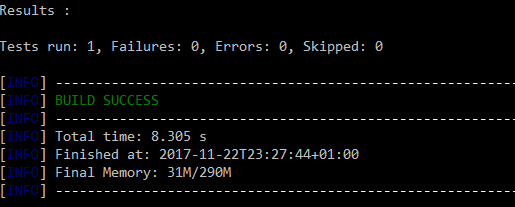
\includegraphics[width=0.6\linewidth]{images/tests}
	\figcaption{Unittest wurde erfolgreich ausgeführt}
\end{minipage}

\subsubsection{Regressiontests}
Die Regressionstests wurden mit \verb|Postman| durchgeführt. Mit Postname können \textbf{POST} und \textbf{GET} requests gesendet und getesten werden.

Das erste Problem auf welches gestoßen wurde war, dass kein \verb|CRSF-Token| vorhanden war beim Versuch ein Post-Request zu senden. Grund ist, das dieser token nur mitgesendet wird, wenn die Seite mit dem Browser aufgerufen wird. Um dieses Problem zu umgehen, wird CRSF in der \verb|WebSecurityConfig| disabled:

\begin{lstlisting}[language=Java]
	.and()
	.csrf().disable();
\end{lstlisting}

Nun konnte eine leere request gesendet werden ohne Fehlermeldungen.

Es wurde eine POST-request erstellt, auf der url \verb|localhost:8080/registration|, welches ein Form mit \textbf{username}, \textbf{password} und \textbf{passwordConfirm} mitsendet, um einen User zu erstellen.

\begin{minipage}{\linewidth}
	\centering
	
\includegraphics[width=0.6\linewidth]{images/test2}
	\figcaption{Es wird ein Form mitgesendet mit Daten}
\end{minipage}

Es können anschließend Tests geschrieben werden, in dem Fall wird überprüft ob auf die welcome Page umgeleitet wurde:

\begin{lstlisting}[language=Java]
pm.test("Status code is 200", function () {
	pm.response.to.have.status(200);
});

pm.test("Body matches string", function () {
	pm.expect(pm.response.text()).to.include("Welcome mwoelfer");
});

\end{lstlisting}

Und bei der Ausführung sollten die Tests funktionieren:

\begin{minipage}{\linewidth}
	\centering
	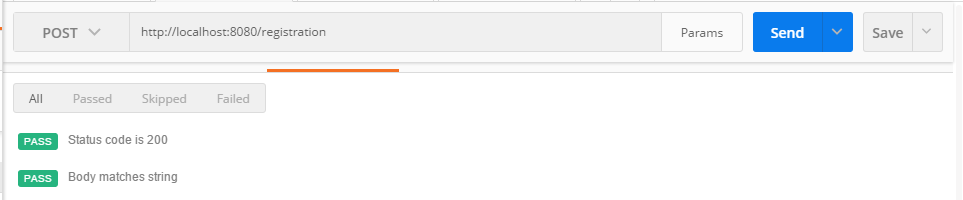
\includegraphics[width=0.6\linewidth]{images/test3}
	\figcaption{Registrations-Test wurde erfolgreich ausgeführt}
\end{minipage}

\clearpage

Es wurde ein weiterer Test für login geschrieben, welcher test ob auf die welcome-page weitergeleitet wird wenn ein Form mit \textbf{user} und \textbf{password} mitgesendet wird:

\begin{minipage}{\linewidth}
	\centering
	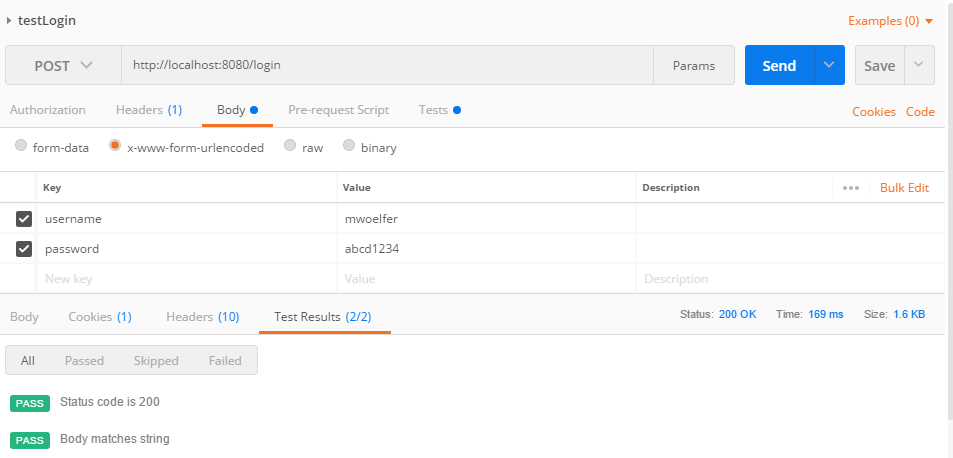
\includegraphics[width=0.6\linewidth]{images/test4}
	\figcaption{Login mit user und password funktioniert}
\end{minipage}